\documentclass[useAMS, usenatbib, a4paper]{mnras}
\pdfsuppresswarningpagegroup=1

\usepackage{graphicx}
\usepackage{microtype}
\usepackage{xcolor}
\usepackage{fixltx2e}
\usepackage{booktabs}
\usepackage{siunitx}
\sisetup{separate-uncertainty = true}
\usepackage{color}
\usepackage{enumerate}
\usepackage{pdflscape}
\usepackage{rotating}
\usepackage{xr-hyper}
\usepackage{hyperref}
\externaldocument[Q-]{quadrics-bowshock}

\usepackage[T1]{fontenc} 
\usepackage[utf8]{inputenc}

% Fonts 
\usepackage{newtxtext}
% Note: newtxmath must come AFTER newtxtext
\usepackage[varvw,smallerops]{newtxmath}

\usepackage{chemgreek}
\activatechemgreekmapping{newtx}

\hypersetup{colorlinks=True, linkcolor=blue!50!black, citecolor=black,
  urlcolor=blue!50!black}

\usepackage{etoolbox}
\robustify\bfseries
\robustify\itshape

%% The following hack solves a problem with
%% ERROR: \pdfendlink ended up in different nesting level than \pdfstartlink.
%% See https://tex.stackexchange.com/a/249743
\makeatletter
\patchcmd\@combinedblfloats{\box\@outputbox}{\unvbox\@outputbox}{}{%
  \errmessage{\noexpand\@combinedblfloats could not be patched}%
}%
\makeatother

%% Bold italic
\newcommand\hmmax{0}            % we don't need heavy fonts
\newcommand\bmmax{1}            % reduce use of math alphabets for bold
\usepackage{bm}

%% Bundled custom packages
\usepackage{aastex-compat}

\title
% {No radiation supported dust wave around \(\sigma\) Orionis}
% OR
{Is the dusty bow shock around \(\sigma\) Orionis driven by an enclosed proplyd?}

\newcommand\AddressCRyA{Instituto de Radioastronom\'{\i}a y Astrof\'{\i}sica,
  Universidad Nacional Aut\'onoma de M\'exico, Apartado Postal 3-72,
  58090 Morelia, Michoac\'an, M\'exico}
\author[Henney \& Arthur]{
  William J. Henney \& S. Jane Arthur\\
  \AddressCRyA
}

% These dates will be filled out by the publisher
\date{Accepted XXX. Received YYY; in original form ZZZ}

% Enter the current year, for the copyright statements etc.
\pubyear{2017}
\DeclareMathOperator{\sgn}{sgn}
\DeclareMathOperator{\Sin}{\mathcal{S}}
\DeclareMathOperator{\Cos}{\mathcal{C}}
\DeclareMathOperator{\Cot}{\mathcal{T}}
\DeclareMathOperator{\GammaFunc}{\Gamma}
\newcommand\w{\ensuremath{\mathrm{w}}}
\newcommand\C{\ensuremath{\mathrm{c}}}
\providecommand{\abs}[1]{\lvert#1\rvert}
\providecommand{\Abs}[1]{\left\lvert#1\right\rvert}
\newcommand\TODO[1]{%
  \begin{center}
    \framebox{\parbox{0.8\linewidth}{
        \texttt{\footnotesize\color{red} #1}}}
  \end{center}}

\newcommand\uvec[1]{\bm{\hat{#1}}}
\newcommand\T{_{\mathrm{\scriptscriptstyle T}}}

\newcommand\Qp{\ensuremath{Q_{\text{p}}}}
\newcommand{\grain}{\ensuremath{_{\text{d}}}}
\newcommand{\B}{\ensuremath{_{\scriptscriptstyle\text{B}}}}
\newcommand{\alfven}{\ensuremath{_{\scriptscriptstyle\text{A}}}}
\newcommand{\xsec}{\ensuremath{\sigma\grain}}
\newcommand\frad{\ensuremath{f_{\text{rad}}}}
\newcommand\fmax{\ensuremath{f_{\text{max}}}}
\newcommand\thm{\ensuremath{\theta_{\text{m}}}}
\newcommand\drag{\ensuremath{_{\text{drag}}}}
\newcommand{\gas}{\ensuremath{_{\text{gas}}}}
\newcommand{\drift}{\ensuremath{_{\text{drift}}}}
\newcommand\rad{\ensuremath{_{\text{rad}}}}
\newcommand\Rmin{\ensuremath{R_{\scriptscriptstyle\text{min}}}}
% Why do I need both of these?
\newcommand\sound{\ensuremath{c_{\text{s}}}}
\newcommand\soundspeed{\ensuremath{c_{\text{s,gas}}}}
\newcommand\starstar{\ensuremath{_{**}}}
\newcommand\hii{\ion{H}{ii}}


\defcitealias{Tarango-Yong:2018a}{Paper~I}
\newcommand\PaperI{\citetalias{Tarango-Yong:2018a}}


\begin{document}
\label{firstpage}
\pagerange{\pageref{firstpage}--\pageref{lastpage}}
\maketitle
\begin{abstract}
  We critically evaluate the role of radiation and hydrodynamics in
  providing internal support for the bow-shaped infrared arc around
  the massive triple star system \(\sigma\)~Ori Aa/Ab/B in the IC434 \hii{}
  region.  We present evidence for hydrogen recombination line
  emission from the arc, which demonstrates that it cannot be a dust
  wave in which the grains have separated from the gas, as has been
  previously claimed.  On the other hand, we show that the fraction of
  the stellar luminosity trapped by the arc is insufficient for it to
  be supported by radiation if the grains and gas are well coupled.
  Therefore, the arc must be supported by the ram pressure of an
  internal wind.  However, the stellar wind from the OB stars in the
  \(\sigma\)~Ori Aa/Ab/B system are too weak by more than an order of
  magnitude.  We propose instead that it is the photoevaporated disk
  wind from the enclosed proplyd IRS~1B that provides the ram pressure
  support for the bow.
\end{abstract}

\begin{keywords}
  circumstellar matter -- radiation: dynamics -- stars: winds, outflows
\end{keywords}

\section{Observational case studies}
\label{sec:case-studies}

In observational studies of bow-shaped arcs around OB stars, it is
frequently assumed that all such objects are wind-supported bow shocks
(e.g., \citealp{Kobulnicky:2016a}). Our results from
\S~\ref{sec:strong-gas-grain} show that this is indeed a fair
assumption in the absence of gas-grain decoupling, so long as the
ambient density is less than about \SI{100}{cm^{-3}} (see
Fig.~\ref{fig:zones-v-n-plane}). In other words, most OB stars
interacting with the diffuse interstellar medium are probably in the
wind bow shock regime.  Therefore, to find examples of
radiation-supported bow waves and bow shocks it is necessary to look
at arcs inside \hii{} regions and star-forming clouds, where the
ambient densities are much higher.

\subsection{Evidence for radiation-supported bows}

One potentially promising sample is the Carina mid-infrared bow shocks
\citep{Sexton:2015b}.   are in a high density environment,
\SI{1000}{cm^{-3}}, so they may be bow waves.  There seems to be
spectral types for most of them: B0 (but supergiant) to O7.  Sizes are
3 to 12 arcsec, which at Carina (\SI{2.3}{kpc}) is
\SIrange{0.033}{0.134}{pc}.

Amazingly, the size/density combination gives regions that overlap
with the dust wave region for both the \SI{20}{M_\odot} and \SI{40}{M_\odot}
case.  And implying velocities of \SIrange{30}{50}{km.s^{-1}}.  This
is more believable than the \SI{10}{km.s^{-1}} that they quote, since
that would not give a shock at all.  This would imply
\(\tau > \eta \approx 0.1\), so the bow luminosity should be 10\% of the star
luminosity, so getting on for \SI{e4}{L_\odot}.

Two small bows in M42:

\newcommand{\thD}{\(\theta^1\)\,Ori~D}
\th1D{} (Ney--Allen nebula) \citep{Robberto:2005a}

LP~Ori: B1.5V star, like our \SI{10}{M_\odot} example. Radius about
\(3''\), so 0.005 pc.  With \(v = 80\) that would clearly be a dust
wave and would require \SIrange{100}{1000}{cm^{-3}}. Gaia distance \SI{408 +- 11}{pc}


Ones that Ochsendorf claims are dust waves (Narrator: they aren't).


\begin{figure*}
  \centering
  \includegraphics[width=\linewidth]{figs/orion-LP-and-th1D-color}
  \caption{Bows driven by the OB stars \thD{} and LP~Ori in the Orion
    Nebula.  (a)~Large-scale infrared view of the Orion Molecular
    Cloud.  Red, green, and blue intensity show respectively Herschel
    PACS observations at \SIlist{160; 70}{\um}, and Spitzer IRAC
    observations at \SI{8}{\um}.  Red traces thermal emission from
    cool dust (\(T < \SI{30}{K}\)) in the dense molecular filament.
    Green traces thermal emission from warmer dust
    (\(T \approx \SI{40}{K}\)) in the neutral PDR, which is heated by
    far-ultraviolet radiation from the OB stars in the cluster. Blue
    traces emission from PAH \SIlist{7.6;7.85}{\um} bands in the same
    neutral PDR plus thermal emission from hotter dust
    (\(T > \SI{100}{K}\)), which is found inside the ionized \hii{}
    region.  (b)~Zoom on the central parsec of the Orion Nebula (M42),
    showing short-wavelength mid-infrared emission from Spitzer IRAC
    observations (\SIlist{8.0;5.8;4.5}{\um}).  Red shows the same as
    blue in panel~a.  Green show predominantly the \SI{6.2}{\um} PAH
    band.  Blue shows mainly stellar photospheric emission, plus a
    minor contribution due to the Br~\(\alpha\) emission line from ionized
    gas. Some major components of the nebula are labelled: the
    Trapezium cluster, which contains the majority of the massive
    stars; the Kleinmann-Low reflection nebula, illuminated by massive
    stars embedded in the molecular filament; the Orion Bar, a
    prominent edge-on ionization front and PDR.  (c)~Zoom on the
    central \SI{0.1}{pc} of the Trapezium cluster, showing longer
    wavelength mid-infrared emission from UKIRT MAX
    (\SIlist{19.7;10.1}{\um}).  In this central zone, these
    wavelengths (shown in red and green) are dominated by warm
    (\SIrange{100}{300}{K}) silicate grains, while the IRAC
    \SI{5.8}{\um} emission (blue) shows stellar photospheres and the
    very warmest dust.}
  \label{fig:orion-bows}
\end{figure*}

\begin{figure*}
  \centering
  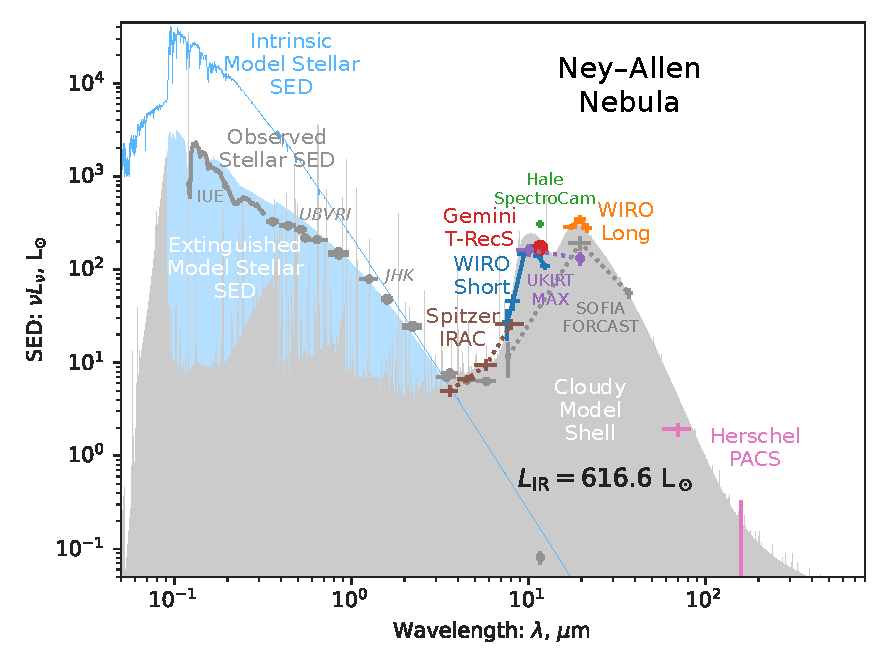
\includegraphics[width=\linewidth]{figs/ney-allen-sed-edited}
  \caption{Ultraviolet-to-infrared spectral energy distribution of the Ney--Allen
    nebula that surrounds \thD. }
  \label{fig:ney-allen-sed}
\end{figure*}


\begin{figure*}
  \centering
  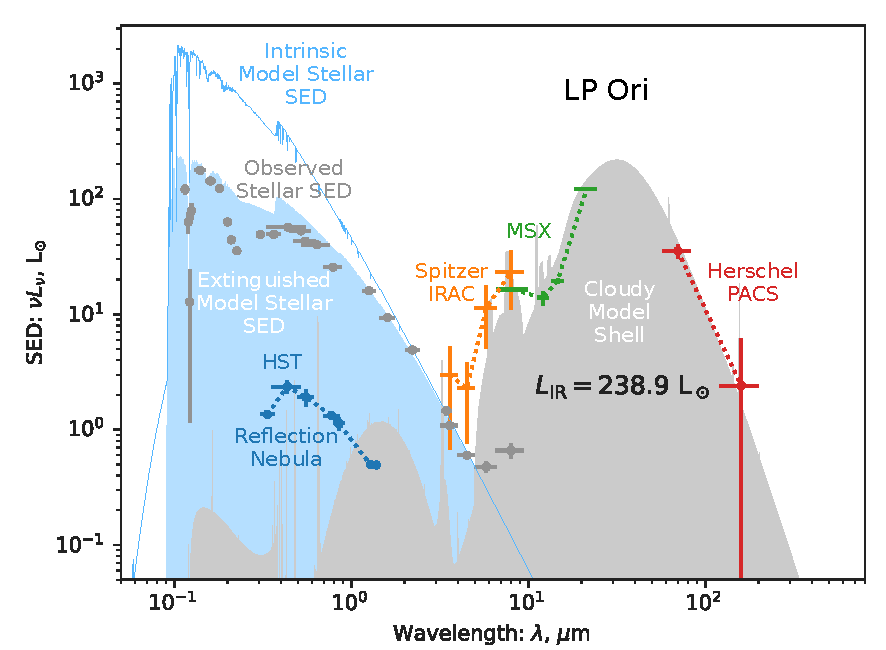
\includegraphics[width=\linewidth]{figs/lp-ori-sed-edited}
  \caption{Ultraviolet-to-infrared spectral energy distribution of LP~Ori
    and associated nebula. }
  \label{fig:lp-ori-sed}
\end{figure*}

\begin{figure}
  \centering
  \includegraphics[width=\linewidth]{figs/lp-ori-wfpc2-continuum-subtract}
  \caption{Narrow-band images of LP Ori nebula }
  \label{fig:lp-ori-sed}
\end{figure}

% Model shell-R001-n27-LP_Ori20Bz5 from cloudy-dust-charging
The Cloudy model for LP Ori


%%% Local Variables:
%%% mode: latex
%%% TeX-master: "two-orions-bow"
%%% End:

\bibliographystyle{mnras}
\bibliography{bowshocks-biblio}

% Don't change these lines
\bsp	% typesetting comment
\label{lastpage}
\end{document}

%%% Local Variables:
%%% mode: latex
%%% TeX-master: t
%%% End:
